\documentclass[10pt, aspectratio=169]{beamer}

\usetheme{Boadilla}
\usecolortheme{default}

% Configuration des informations globales pour le pied de page automatique
\title[Optimisation NLP]{Étude des Méthodes de Gradient Adaptatif en NLP}
\author[M. BOULATAR \& M. A. GHAZLI]{Mouad BOULATAR, Mohamed Amine GHAZLI, Ayoub HAMROUDI, Jad MOUSLIM}
\institute[FSBM]{Faculté des Sciences Ben M'sik}
\date[Juin 2026]{Juin 2026}

% Suppression des barres classiques de navigation inutiles
\setbeamertemplate{navigation symbols}{}

% Packages indispensables pour la gestion des couleurs et graphiques
\usepackage{xcolor}
\usepackage{graphicx}
\usepackage{fontawesome5}
\usepackage{tikz}
\usepackage{booktabs}

% Configuration des langues
\usepackage[T1]{fontenc}
\usepackage[utf8]{inputenc}
\usepackage[french]{babel}

% Couleurs "Startup / Deep Tech"
\definecolor{StartupBlue}{HTML}{34495E}
\definecolor{StartupCyan}{HTML}{16A085}
\definecolor{BadgeGrey}{HTML}{EAEDED}

% Application des styles aux blocs Beamer
\setbeamercolor{structure}{fg=StartupBlue}
\setbeamercolor{palette primary}{bg=StartupBlue, fg=white}
\setbeamercolor{palette secondary}{bg=StartupCyan, fg=white}
\setbeamercolor{block title}{bg=StartupBlue!10, fg=StartupBlue}
\setbeamercolor{block body}{bg=StartupBlue!5, fg=black}
\setbeamercolor{alerted text}{fg=StartupCyan}

% ============================================================
% SUPPRESSION COMPLETE DU HEADER (EN-TÊTE)
% ============================================================
\setbeamertemplate{headline}{}

% ============================================================
% FOOTER PERSONNALISÉ
% ============================================================
\setbeamertemplate{footline}{%
    \leavevmode%
    \hbox{%
        \begin{beamercolorbox}[wd=.333\paperwidth,ht=2.5ex,dp=1.125ex,leftskip=.3cm,rightskip=.3cm]{author in head/foot}%
            \usebeamerfont{author in head/foot}%
            \color{white}\textbf{Groupe 16 — Data Science And Big Data}
        \end{beamercolorbox}%
        \begin{beamercolorbox}[wd=.334\paperwidth,ht=2.5ex,dp=1.125ex,leftskip=.3cm,rightskip=.3cm,center]{title in head/foot}%
            \usebeamerfont{title in head/foot}%
            \color{white}\textbf{Gradient Adaptatif en NLP}
        \end{beamercolorbox}%
        \begin{beamercolorbox}[wd=.333\paperwidth,ht=2.5ex,dp=1.125ex,leftskip=.3cm,rightskip=.3cm,right]{date in head/foot}%
            \usebeamerfont{date in head/foot}%
            \color{white}\textbf{Juin 2026}
            \hspace{0.5cm}
            \insertframenumber\,/\,\inserttotalframenumber
        \end{beamercolorbox}%
    }%
    \vskip0pt%
}
% ============================================================
% PAGE DE GARDE AVEC LOGOS (SANS HEADER NI FOOTER)
% ============================================================
\setbeamertemplate{title page}{
    \begin{tikzpicture}[remember picture, overlay]
        % Fond 100% blanc pur
        \fill[white] (current page.south west) rectangle (current page.north east);

        % ============================================================
        % LOGOS EN HAUT DE PAGE
        % ============================================================
        \node[anchor=north west] at ([xshift=0.6cm, yshift=-0.4cm]current page.north west) {
            
\includegraphics[height=1.2cm]{logo_fsbm.png}
        };

        \node[anchor=north east] at ([xshift=-0.6cm, yshift=-0.4cm]current page.north east) {
            
\includegraphics[height=1.2cm]{logo_master.png}
        };

        % ============================================================
        % BADGE "PROJET DE FIN DE MODULE"
        % ============================================================
        \node[anchor=south, fill=StartupBlue!8, text=StartupBlue, rounded corners=3pt, inner sep=4pt, font=\bfseries\tiny]
            at ([yshift=2.7cm]current page.center)
            {\faBrain \quad PROJET FIN MODULE ALGORITHMES D'OPTIMISATION};

        % ============================================================
        % TITRE PRINCIPAL
        % ============================================================
        \node[anchor=north, text width=0.9\textwidth, align=center]
            at ([yshift=2.45cm]current page.center) {
            {\Huge \bfseries \color{StartupBlue} Étude\ des\ Méthodes\ de} \\[4pt]
            {\Huge \bfseries \color{StartupCyan} Gradient\ Adaptatif\ en\ NLP}
        };
	

	 \vspace{1cm}
        % Sous-titre
        \node[anchor=north, text width=0.85\textwidth, align=center]
            at ([yshift=0.55cm]current page.center) {
            {\footnotesize \color{gray!60!black} Comparaison de 5 optimiseurs pour le fine-tuning de DistilBERT sur IMDB}
        };

        % Ligne décorative
        \draw[StartupCyan, line width=2pt] ([xshift=-1.5cm, yshift=0.05cm]current page.center) -- ([xshift=1.5cm, yshift=0.05cm]current page.center);

        % ============================================================
        % STACK TECHNIQUE (Technologies Clés)
        % ============================================================
        \node[anchor=north, text width=0.9\textwidth, align=center]
            at ([yshift=-0.05cm]current page.center) {
            {\scriptsize \color{gray!80!black} \bfseries \faTools \quad Technologies\ Clés\ : } \\[5pt]
            \tikz[baseline=(X.base)]\node[fill=BadgeGrey, text=StartupBlue, rounded corners=2pt, inner sep=3pt, font=\tiny\bfseries](X){\faFire\ PyTorch}; \quad
            \tikz[baseline=(X.base)]\node[fill=BadgeGrey, text=StartupBlue, rounded corners=2pt, inner sep=3pt, font=\tiny\bfseries](X){\faRobot\ HuggingFace}; \quad
            \tikz[baseline=(X.base)]\node[fill=BadgeGrey, text=StartupBlue, rounded corners=2pt, inner sep=3pt, font=\tiny\bfseries](X){\faBrain\ DistilBERT}; \quad
            \tikz[baseline=(X.base)]\node[fill=BadgeGrey, text=StartupBlue, rounded corners=2pt, inner sep=3pt, font=\tiny\bfseries](X){\faGoogle\ Colab}; \quad
            \tikz[baseline=(X.base)]\node[fill=BadgeGrey, text=StartupBlue, rounded corners=2pt, inner sep=3pt, font=\tiny\bfseries](X){\faChartLine\ Scikit-learn};
        };

        % ============================================================
        % INFORMATIONS EN BAS DE PAGE
        % ============================================================
        % Gauche : Étudiants
        \node[anchor=south west, text width=0.32\textwidth, align=left]
            at ([xshift=0.8cm, yshift=0.35cm]current page.south west) {
            {\scriptsize \color{gray} \faUserGraduate \quad Réalisé par :} \\[2pt]
            {\small \bfseries \color{StartupBlue} Mouad BOULATAR} \\
            {\small \bfseries \color{StartupBlue} Mohamed Amine GHAZLI} \\
            {\small \bfseries \color{StartupBlue} Ayoub HAMROUDI} \\
            {\small \bfseries \color{StartupBlue} Jad MOUSLIM} \\
        };

        % Centre : Encadrement (Placé en bas)
        \node[anchor=south, text width=0.32\textwidth, align=center]
            at ([yshift=0.75cm]current page.south) {
            {\scriptsize \color{gray} \faUserTie \quad Supervisé par :} \\[2pt]
            {\small \bfseries \color{StartupBlue} Pr. Faouzia BENABBOU}
        };

        % Droite : Date
        \node[anchor=south east, text width=0.32\textwidth, align=right]
            at ([xshift=-0.8cm, yshift=0.75cm]current page.south east) {
            {\scriptsize \color{gray} \faCalendar \quad Date :} \\[2pt]
            {\small \bfseries \color{StartupBlue} Juin 2026} \\
            {\tiny \color{gray} Soutenance orale}
        };
    \end{tikzpicture}
}

\begin{document}

% ============================================================
% PAGE 1 : PAGE DE GARDE (SANS HEADER/FOOTER)
% ============================================================
\begin{frame}[plain]
    \titlepage
\end{frame}
% ============================================================
% PAGE 2 : PLAN DE LA PRÉSENTATION
% ============================================================
\begin{frame}{Plan de la Présentation}
    \vspace{0.2cm}
    \begin{columns}[t]
        \begin{column}{0.48\textwidth}
            \begin{itemize}
                \setlength{\itemsep}{12pt}
                \item[\color{StartupCyan}\bfseries 01] Contexte \& Problématique
                \item[\color{StartupCyan}\bfseries 02] Optimiseurs Étudiés
                \item[\color{StartupCyan}\bfseries 03] Méthodologie \& Architecture
                \item[\color{StartupCyan}\bfseries 04] Résultats Principaux
            \end{itemize}
        \end{column}

        \begin{column}{0.48\textwidth}
            \begin{itemize}
                \setlength{\itemsep}{12pt}
                \item[\color{StartupCyan}\bfseries 05] Analyses de Sensibilité
                \item[\color{StartupCyan}\bfseries 06] Discussion Critique
                \item[\color{StartupCyan}\bfseries 07] Conclusion \& Recommandations
            \end{itemize}
        \end{column}
    \end{columns}
\end{frame}

% ============================================================
% PAGE 3 : TRANSITION CHAPITRE 1
% ============================================================
\section{Contexte \& Problématique}
\begin{frame}
    \begin{tikzpicture}[remember picture, overlay]
        \fill[white] (current page.south west) rectangle (current page.north east);
        \node[text=StartupCyan!10, font=\fontsize{100}{100}\selectfont\bfseries, anchor=center] at ([xshift=-4cm, yshift=0.5cm]current page.center) {01};
        \node[fill=StartupCyan!10, text=StartupCyan, rounded corners=3pt, inner sep=5pt, font=\bfseries\tiny, anchor=west] at ([xshift=1.5cm, yshift=1.2cm]current page.west) {\faCompass\quad CHAPITRE PREMIER};
        \node[text width=0.75\textwidth, anchor=west, align=left] at ([xshift=1.5cm, yshift=0.2cm]current page.west) {
            {\Huge \bfseries \color{StartupBlue} Contexte \& Problématique} \\[6pt]
            {\Large \color{StartupCyan} Le Défi de l'Optimisation pour les Transformers}
        };
        \draw[StartupBlue!20, line width=1.5pt] ([xshift=1.5cm, yshift=-0.8cm]current page.west) -- ([xshift=1.5cm, yshift=-2.6cm]current page.west);
        \node[text width=0.7\textwidth, anchor=west, align=left] at ([xshift=1.8cm, yshift=-1.7cm]current page.west) {
            {\scriptsize \color{gray} \bfseries Au programme :} \\[4pt]
            {\footnotesize \color{StartupBlue} \faArrowCircleRight \quad Domination des Transformers en NLP} \\
            {\footnotesize \color{StartupBlue} \faArrowCircleRight \quad Sensibilité au choix de l'optimiseur} \\
            {\footnotesize \color{StartupBlue} \faArrowCircleRight \quad Objectifs scientifiques du projet}
        };
    \end{tikzpicture}
\end{frame}

% ============================================================
% PAGE 4 : CONTENU 1 — CONTEXTE & PROBLÉMATIQUE
% ============================================================
\begin{frame}{Contexte \& Problématique}
    \vspace{0.1cm}
    \begin{columns}[t]
        \begin{column}{0.48\textwidth}
            \begin{block}{\faExclamationTriangle\quad Constat \& Problématique}
                \vspace{0.2cm}
                \footnotesize
                Les architectures \textbf{Transformer} (BERT, DistilBERT) dominent le NLP moderne, mais leur fine-tuning reste sensible au choix de l'optimiseur.
                \\[8pt]
                Les gradients sont \textbf{bruités}, l'espace des paramètres est de \textbf{très haute dimension}, et la performance dépend fortement du \textit{learning rate}.
                \vspace{0.2cm}
            \end{block}
        \end{column}
        \begin{column}{0.48\textwidth}
            \vspace{0.1cm}
            {\large \bfseries \color{StartupBlue} Objectifs du Projet :}
            \vspace{0.3cm}
            \begin{itemize}
                \setlength{\itemsep}{10pt}
                \item[\color{StartupCyan}\faRunning] \textbf{Vitesse de convergence}
                \item[\color{StartupCyan}\faWaveSquare] \textbf{Stabilité de l'apprentissage}
                \item[\color{StartupCyan}\faMemory] \textbf{Consommation mémoire GPU}
                \item[\color{StartupCyan}\faChartLine] \textbf{Capacité de généralisation}
            \end{itemize}
        \end{column}
    \end{columns}
\end{frame}

% ============================================================
% PAGE 5 : TRANSITION CHAPITRE 2
% ============================================================
\section{Optimiseurs Étudiés}
\begin{frame}
    \begin{tikzpicture}[remember picture, overlay]
        \fill[white] (current page.south west) rectangle (current page.north east);
        \node[text=StartupCyan!10, font=\fontsize{100}{100}\selectfont\bfseries, anchor=center] at ([xshift=-4cm, yshift=0.5cm]current page.center) {02};
        \node[fill=StartupCyan!10, text=StartupCyan, rounded corners=3pt, inner sep=5pt, font=\bfseries\tiny, anchor=west] at ([xshift=1.5cm, yshift=1.2cm]current page.west) {\faSitemap\quad CHAPITRE DEUXIÈME};
        \node[text width=0.75\textwidth, anchor=west, align=left] at ([xshift=1.5cm, yshift=0.2cm]current page.west) {
            {\Huge \bfseries \color{StartupBlue} Les Optimiseurs Étudiés} \\[6pt]
            {\Large \color{StartupCyan} 5 Algorithmes, 5 Philosophies}
        };
        \draw[StartupBlue!20, line width=1.5pt] ([xshift=1.5cm, yshift=-0.8cm]current page.west) -- ([xshift=1.5cm, yshift=-2.6cm]current page.west);
        \node[text width=0.7\textwidth, anchor=west, align=left] at ([xshift=1.8cm, yshift=-1.7cm]current page.west) {
            {\scriptsize \color{gray} \bfseries Au programme :} \\[4pt]
            {\footnotesize \color{StartupBlue} \faArrowCircleRight \quad SGD, AdamW, AdaFactor} \\
            {\footnotesize \color{StartupBlue} \faArrowCircleRight \quad LAMB \& Lion} \\
            {\footnotesize \color{StartupBlue} \faArrowCircleRight \quad Mécanismes clés de chacun}
        };
    \end{tikzpicture}
\end{frame}

% ============================================================
% PAGE 6 : CONTENU 2 — LES 5 OPTIMISEURS
% ============================================================
\begin{frame}{Les 5 Optimiseurs Étudiés}
    \vspace{0.1cm}
    \begin{columns}[t]
        \begin{column}{0.55\textwidth}
            \footnotesize
            \begin{tabular}{lll}
                \toprule
                \textbf{\color{StartupBlue}Optimiseur} & \textbf{\color{StartupBlue}Type} & \textbf{\color{StartupBlue}Année} \\
                \midrule
                SGD + Momentum & Non-adaptatif & Classique \\
                AdamW & Weight decay découplé & 2017 \\
                AdaFactor & Mémoire réduite & 2018 \\
                LAMB & Trust ratio par couche & 2019 \\
                Lion & Sign momentum & 2023 \\
                \bottomrule
            \end{tabular}
        \end{column}
        \begin{column}{0.43\textwidth}
            \begin{alertblock}{\faLightbulb\quad Mécanisme clé}
                \scriptsize
                \textbf{AdaFactor} factorise la matrice des second-moments : mémoire \textbf{sous-linéaire}, idéal pour GPU limités.
                \\[4pt]
                \textbf{Lion} n'utilise que le \textbf{signe} du momentum : très léger en mémoire mais sensible au LR.
            \end{alertblock}
        \end{column}
    \end{columns}
    \vspace{0.3cm}
    \begin{block}{\faInfoCircle\quad En résumé}
        \scriptsize
        \textbf{AdamW} reste la référence stable. \textbf{AdaFactor} économise la mémoire. \textbf{LAMB} cible les très grands batchs. \textbf{Lion} mise sur la simplicité du signe. \textbf{SGD} sert de baseline non-adaptative.
    \end{block}
\end{frame}

% ============================================================
% PAGE 7 : TRANSITION CHAPITRE 3
% ============================================================
\section{Méthodologie \& Architecture}
\begin{frame}
    \begin{tikzpicture}[remember picture, overlay]
        \fill[white] (current page.south west) rectangle (current page.north east);
        \node[text=StartupCyan!10, font=\fontsize{100}{100}\selectfont\bfseries, anchor=center]
            at ([xshift=-4cm, yshift=0.5cm]current page.center) {03};
        \node[fill=StartupCyan!10, text=StartupCyan, rounded corners=3pt, inner sep=5pt, font=\bfseries\tiny, anchor=west]
            at ([xshift=1.5cm, yshift=1.6cm]current page.west)
            {\faFlask\quad CHAPITRE TROISIÈME};
        \node[text width=0.9\textwidth, anchor=west, align=left]
            at ([xshift=1.5cm, yshift=0.5cm]current page.west) {
            {\fontsize{26}{30}\selectfont\bfseries \color{StartupBlue} Méthodologie \& Architecture} \\[4pt]
            {\Large \color{StartupCyan} Protocole Expérimental Standardisé}
        };
        \draw[StartupBlue!20, line width=1.5pt] ([xshift=1.5cm, yshift=-0.4cm]current page.west) -- ([xshift=1.5cm, yshift=-2.4cm]current page.west);
        \node[text width=0.8\textwidth, anchor=west, align=left]
            at ([xshift=1.8cm, yshift=-1.4cm]current page.west) {
            {\scriptsize \color{gray} \bfseries Au programme :} \\[4pt]
            {\footnotesize \color{StartupBlue} \faArrowCircleRight \quad Modèle DistilBERT \& dataset IMDB} \\
            {\footnotesize \color{StartupBlue} \faArrowCircleRight \quad Protocole expérimental fixe} \\
            {\footnotesize \color{StartupBlue} \faArrowCircleRight \quad Pipeline de benchmark}
        };
    \end{tikzpicture}
\end{frame}

% ============================================================
% PAGE 8 : CONTENU — MODÈLE, DATASET & PROTOCOLE
% ============================================================
\begin{frame}{Modèle, Dataset \& Protocole Expérimental}
    \vspace{0.1cm}
    \begin{columns}[c]
        \begin{column}{0.46\textwidth}
            \begin{block}{\faBrain\quad Modèle \& Dataset}
                \scriptsize
                \textbf{DistilBERT} : 66M paramètres, 6 couches Transformer.
                \\[4pt]
                \textbf{IMDB} : 8\,000 train / 2\,000 val. / 2\,000 test, classes équilibrées 50/50.
            \end{block}
            \vspace{0.15cm}
            {\footnotesize \bfseries \color{StartupBlue} Protocole fixe :}
            \begin{itemize}
                \setlength{\itemsep}{4pt}
                \item[\color{StartupCyan}\faSeedling] Seed = 42, 3 epochs
                \item[\color{StartupCyan}\faSlidersH] Batch = 16, LR = 2e-5
                \item[\color{StartupCyan}\faWeightHanging] Weight decay = 0.01, warmup = 10\%
                \item[\color{StartupCyan}\faBolt] Mixed precision (AMP)
            \end{itemize}
        \end{column}

        \begin{column}{0.52\textwidth}
            \begin{center}
                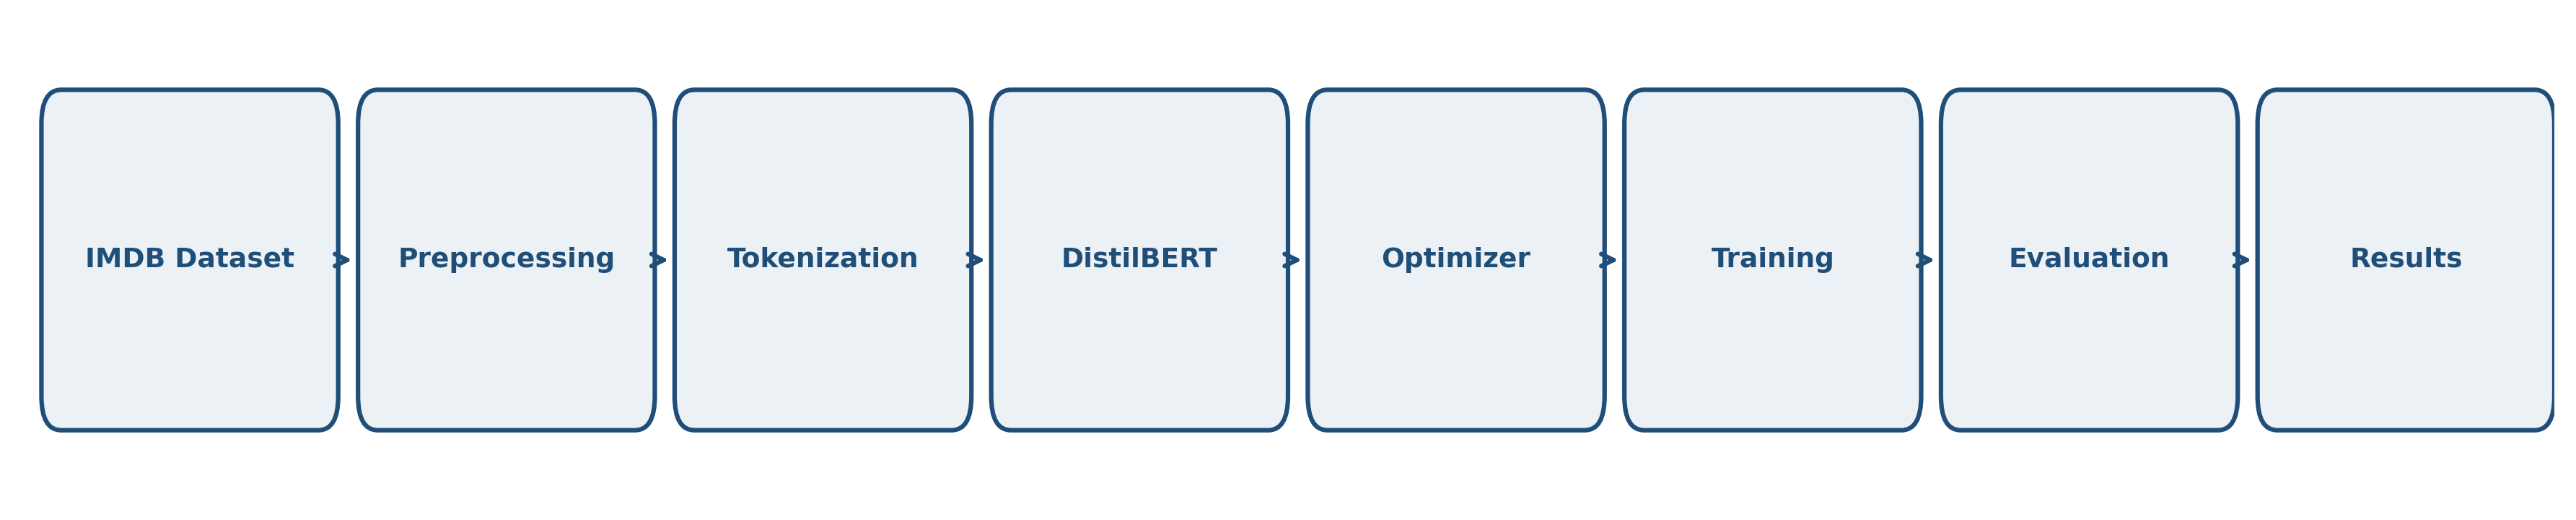
\includegraphics[width=\textwidth, height=0.6\textheight, keepaspectratio]{schema_global_arch.png}
                \\[4pt]
                \tiny \color{gray} \textit{Figure : Architecture globale du pipeline NLP}
            \end{center}
        \end{column}
    \end{columns}
\end{frame}

% ============================================================
% PAGE 9 : CONTENU — PIPELINE EXPÉRIMENTAL
% ============================================================
\begin{frame}{Pipeline Expérimental \& Suivi des Gradients}
    \vspace{0.1cm}
    \begin{columns}[c]
        \begin{column}{0.45\textwidth}
            \begin{block}{\faCogs\quad Benchmark Multi-Optimiseurs}
                \scriptsize
                Chaque optimiseur est évalué sous le \textbf{même protocole} : mêmes données, même seed, mêmes hyperparamètres fixes.
            \end{block}
            \vspace{0.2cm}
            \begin{alertblock}{\faSearch\quad Suivi des gradients}
                \scriptsize
                Norme L2 des gradients mesurée à chaque couche : \textit{Embeddings}, \textit{Layer 0}, \textit{Layer 2}, \textit{Layer 5}, \textit{Classifier}.
            \end{alertblock}
        \end{column}

        \begin{column}{0.53\textwidth}
            \begin{center}
                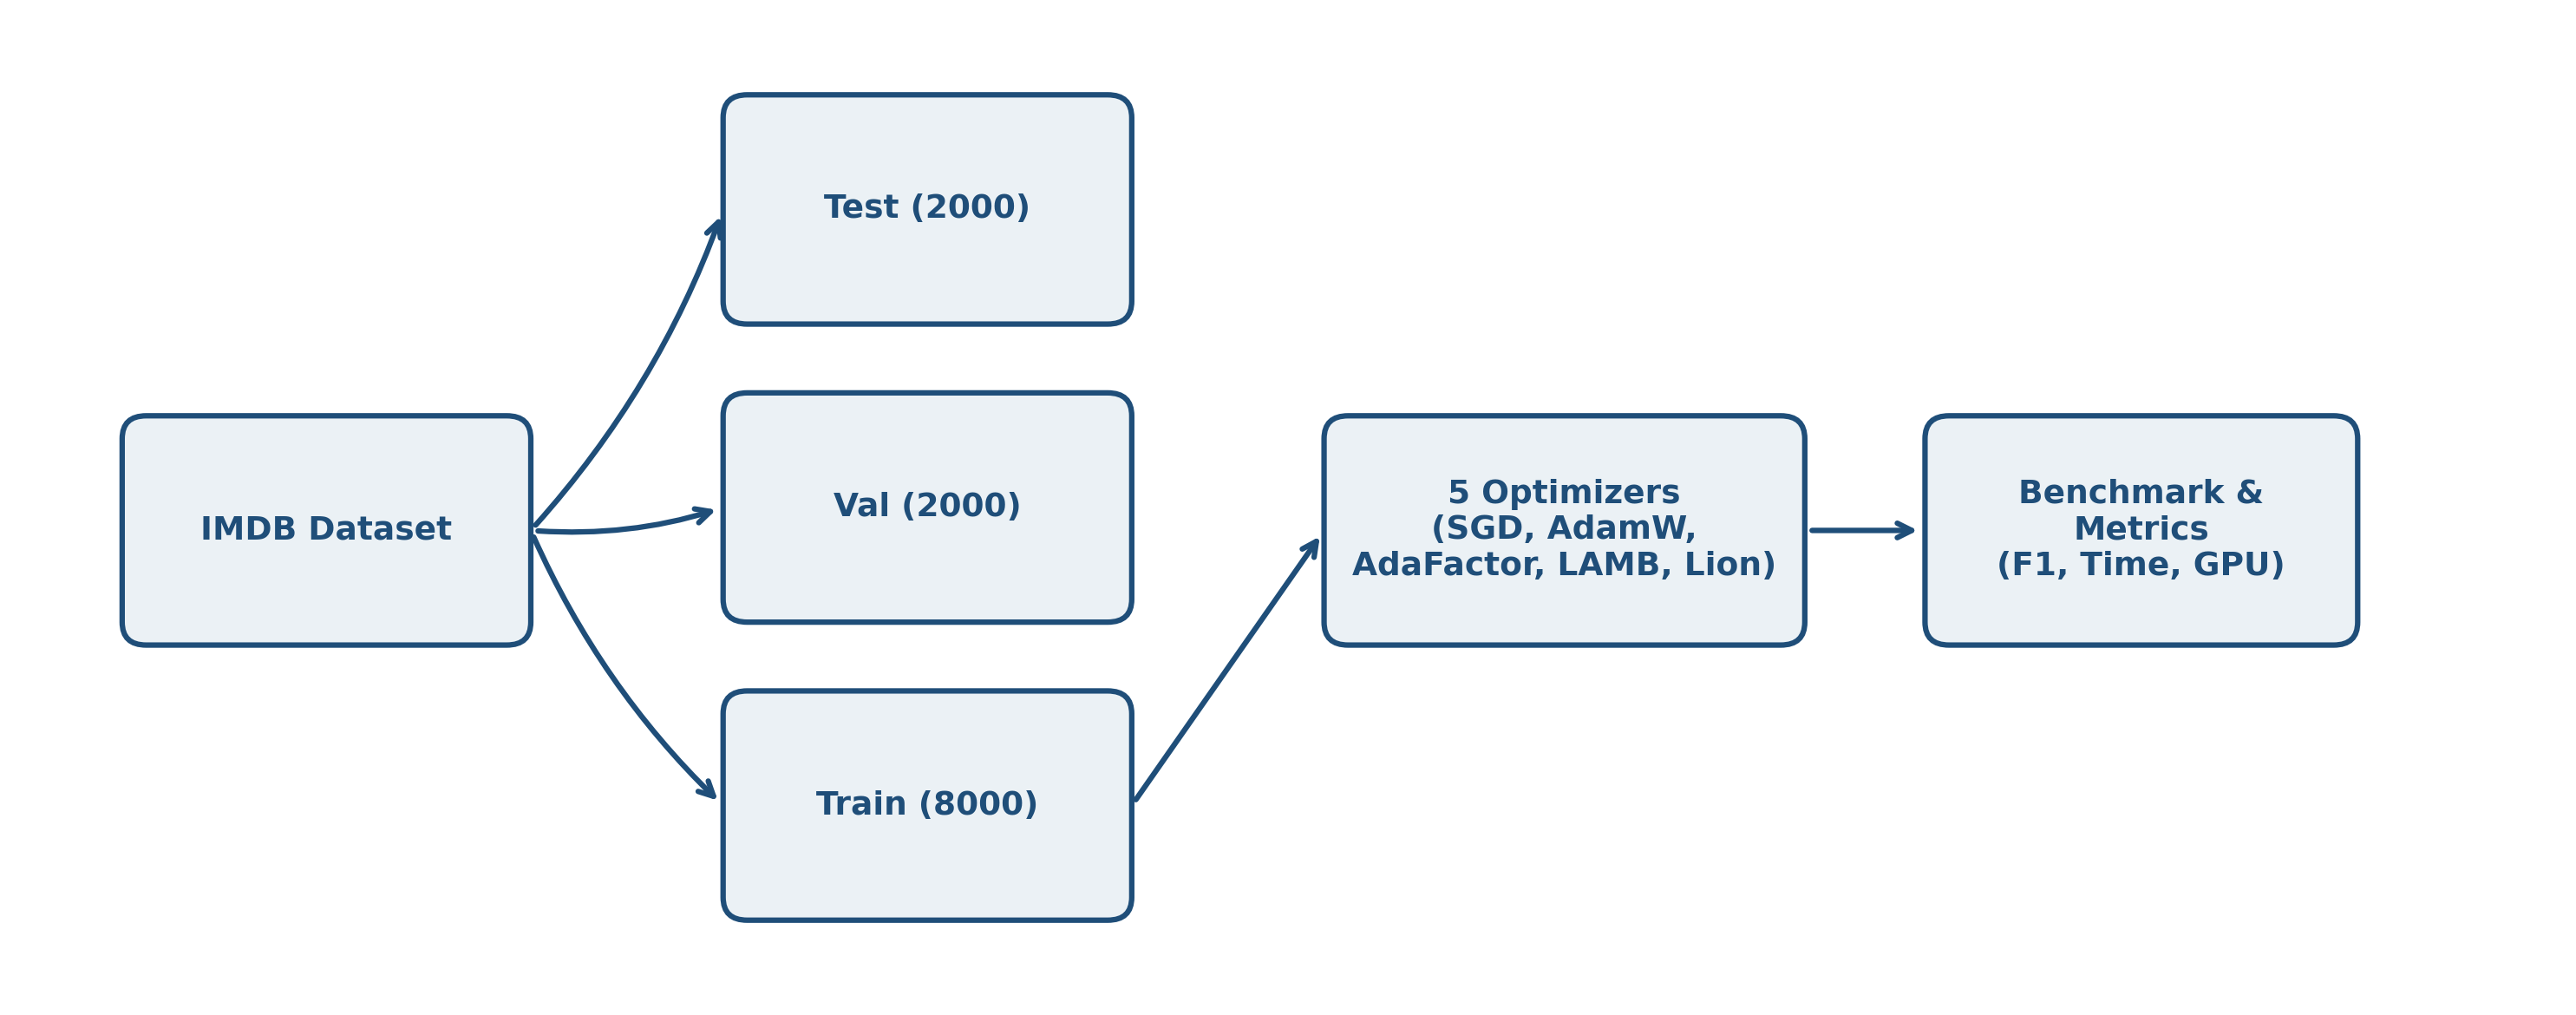
\includegraphics[width=\textwidth, height=0.55\textheight, keepaspectratio]{schema_exp_pipeline.png}
                \\[4pt]
                \tiny \color{gray} \textit{Figure : Pipeline expérimental du benchmark}
            \end{center}
        \end{column}
    \end{columns}
\end{frame}

% ============================================================
% PAGE 10 : TRANSITION CHAPITRE 4
% ============================================================
\section{Résultats Principaux}
\begin{frame}
    \begin{tikzpicture}[remember picture, overlay]
        \fill[white] (current page.south west) rectangle (current page.north east);
        \node[text=StartupCyan!10, font=\fontsize{100}{100}\selectfont\bfseries, anchor=center] at ([xshift=-4cm, yshift=0.5cm]current page.center) {04};
        \node[fill=StartupCyan!10, text=StartupCyan, rounded corners=3pt, inner sep=5pt, font=\bfseries\tiny, anchor=west] at ([xshift=1.5cm, yshift=1.2cm]current page.west) {\faChartBar\quad CHAPITRE QUATRIÈME};
        \node[text width=0.75\textwidth, anchor=west, align=left] at ([xshift=1.5cm, yshift=0.2cm]current page.west) {
            {\Huge \bfseries \color{StartupBlue} Résultats Principaux} \\[6pt]
            {\Large \color{StartupCyan} Benchmark Comparatif des 5 Optimiseurs}
        };
        \draw[StartupBlue!20, line width=1.5pt] ([xshift=1.5cm, yshift=-0.8cm]current page.west) -- ([xshift=1.5cm, yshift=-2.6cm]current page.west);
        \node[text width=0.7\textwidth, anchor=west, align=left] at ([xshift=1.8cm, yshift=-1.7cm]current page.west) {
            {\scriptsize \color{gray} \bfseries Au programme :} \\[4pt]
            {\footnotesize \color{StartupBlue} \faArrowCircleRight \quad Tableau comparatif final} \\
            {\footnotesize \color{StartupBlue} \faArrowCircleRight \quad Courbes de convergence} \\
            {\footnotesize \color{StartupBlue} \faArrowCircleRight \quad Classement des optimiseurs}
        };
    \end{tikzpicture}
\end{frame}

% ============================================================
% PAGE 11 : CONTENU — TABLEAU DE RÉSULTATS
% ============================================================
\begin{frame}{Résultats Principaux — Tableau Comparatif}
    \vspace{0.1cm}
    \begin{columns}[c]
        \begin{column}{0.52\textwidth}
            \footnotesize
            \begin{tabular}{lccc}
                \toprule
                \textbf{\color{StartupBlue}Optim.} & \textbf{\color{StartupBlue}F1} & \textbf{\color{StartupBlue}GPU} & \textbf{\color{StartupBlue}Temps} \\
                \midrule
                \textbf{AdaFactor} & \textbf{89.72\%} & \textbf{1204 MB} & 263.5s \\
                AdamW & 89.53\% & 1724 MB & 250.6s \\
                Lion & 85.99\% & 1468 MB & 243.8s \\
                LAMB & 81.52\% & 1719 MB & 273.3s \\
                SGD+Mom. & 53.79\% & 1458 MB & 235.6s \\
                \bottomrule
            \end{tabular}
            \vspace{0.3cm}
            \begin{alertblock}{\faTrophy\quad Classement Final}
                \scriptsize
                \textbf{1.} AdaFactor \quad \textbf{2.} AdamW \quad \textbf{3.} Lion \\
                \textbf{4.} LAMB \quad \textbf{5.} SGD (échec convergence)
            \end{alertblock}
        \end{column}

        \begin{column}{0.46\textwidth}
            \begin{center}
                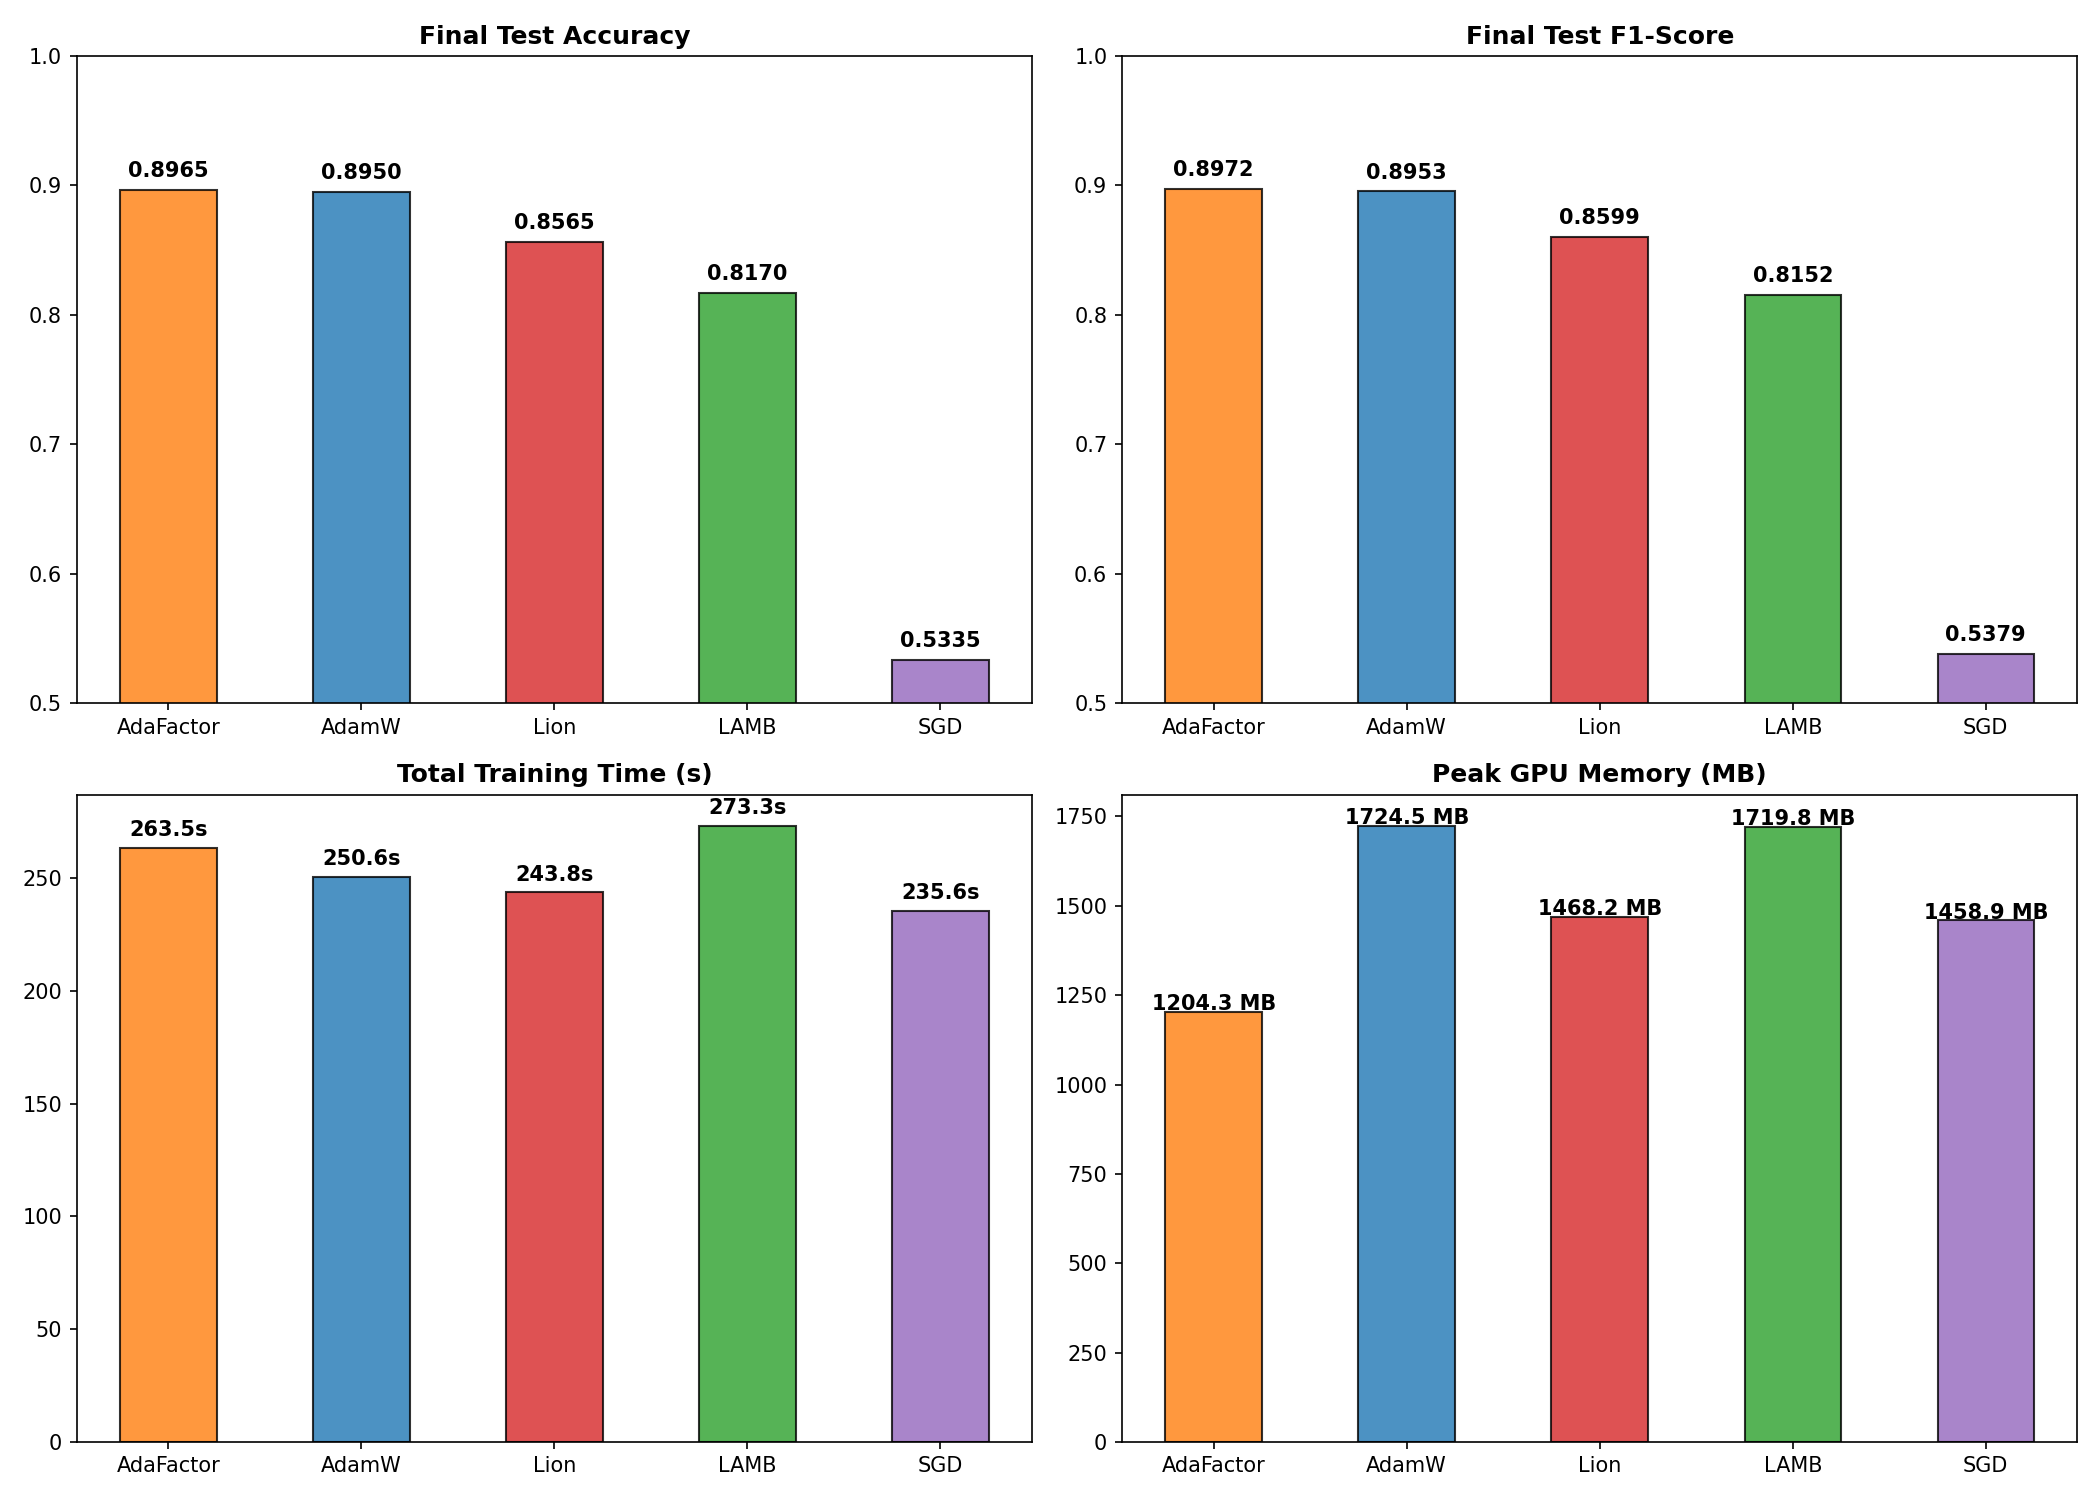
\includegraphics[width=\textwidth, height=0.6\textheight, keepaspectratio]{final_metrics_comparison.png}
                \\[4pt]
                \tiny \color{gray} \textit{Figure : Comparaison finale des métriques}
            \end{center}
        \end{column}
    \end{columns}
\end{frame}

% ============================================================
% PAGE 12 : CONTENU — COURBES DE CONVERGENCE
% ============================================================
\begin{frame}{Courbes de Convergence}
    \vspace{0.1cm}
    \begin{columns}[c]
        \begin{column}{0.40\textwidth}
            \begin{block}{\faChartLine\quad Observations Clés}
                \scriptsize
                \textbf{AdamW \& AdaFactor} : convergence rapide et stable dès l'epoch 1.
                \\[6pt]
                \textbf{SGD} : stagnation, forte variance, échec.
                \\[6pt]
                \textbf{Lion} : léger surapprentissage à l'epoch 3.
                \\[6pt]
                \textbf{LAMB} : convergence lente.
            \end{block}
        \end{column}

        \begin{column}{0.58\textwidth}
            \begin{center}
                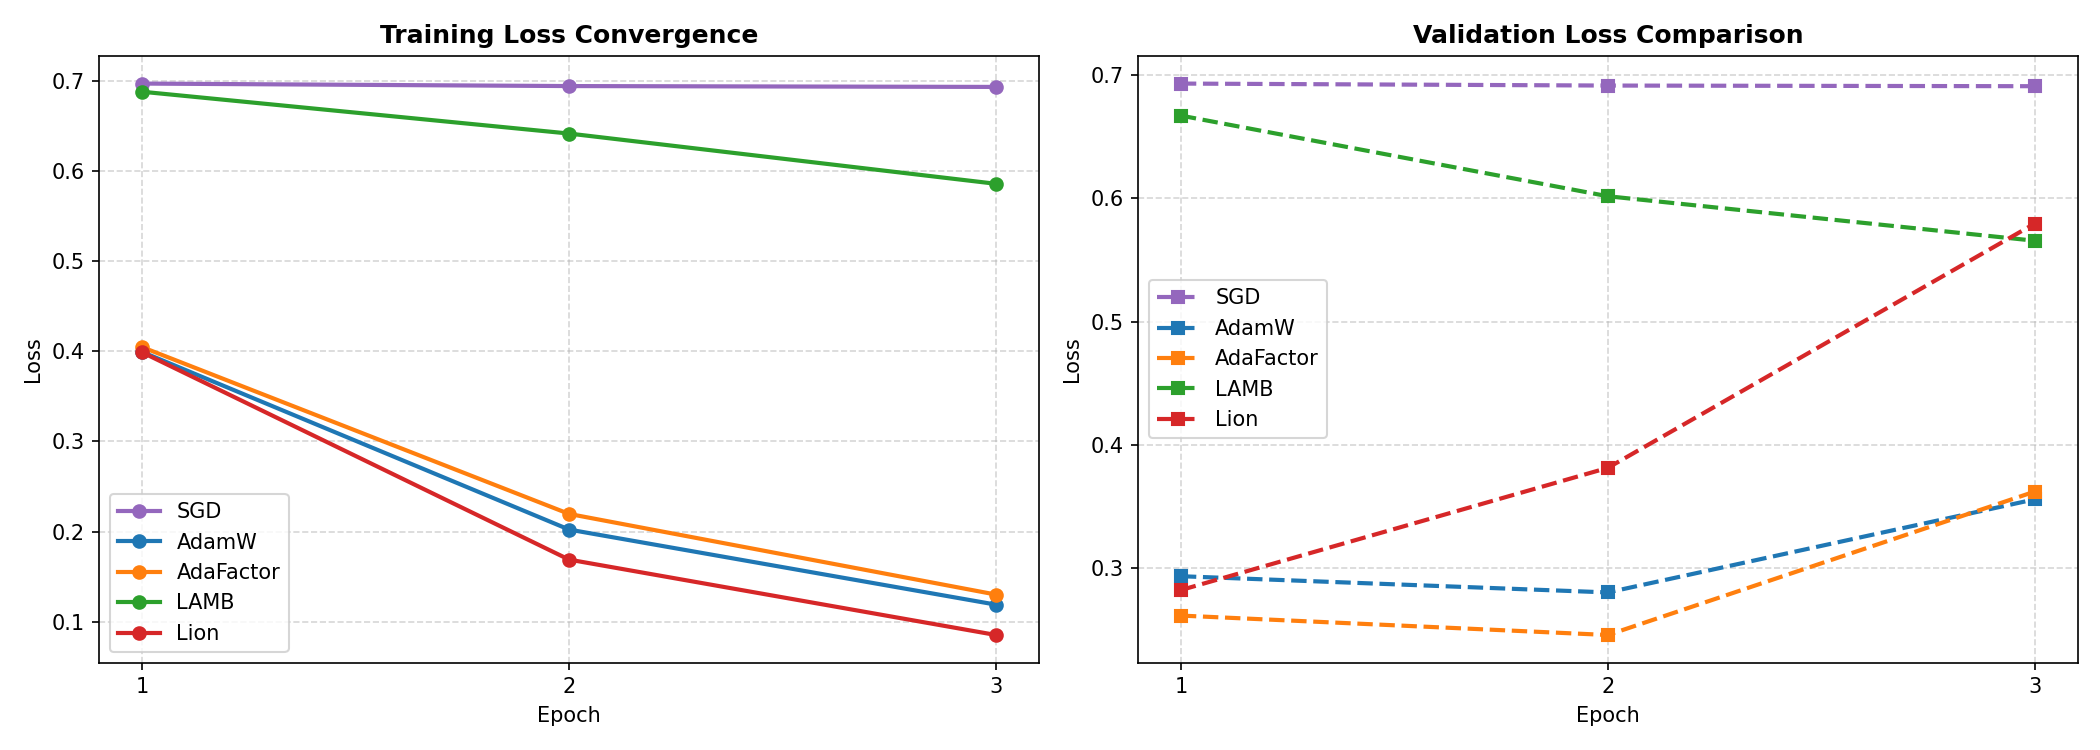
\includegraphics[width=\textwidth, height=0.6\textheight, keepaspectratio]{loss_curves.png}
                \\[4pt]
                \tiny \color{gray} \textit{Figure : Courbes loss train/validation par epoch}
            \end{center}
        \end{column}
    \end{columns}
\end{frame}

% ============================================================
% PAGE 13 : TRANSITION CHAPITRE 5
% ============================================================
\section{Analyses de Sensibilité}
\begin{frame}
    \begin{tikzpicture}[remember picture, overlay]
        \fill[white] (current page.south west) rectangle (current page.north east);
        \node[text=StartupCyan!10, font=\fontsize{100}{100}\selectfont\bfseries, anchor=center]
            at ([xshift=-4cm, yshift=0.5cm]current page.center) {05};
        \node[fill=StartupCyan!10, text=StartupCyan, rounded corners=3pt, inner sep=5pt, font=\bfseries\tiny, anchor=west]
            at ([xshift=1.5cm, yshift=1.7cm]current page.west)
            {\faBalanceScale\quad CHAPITRE CINQUIÈME};
        \node[text width=0.9\textwidth, anchor=west, align=left]
            at ([xshift=1.5cm, yshift=0.5cm]current page.west) {
            {\Huge \bfseries \color{StartupBlue} Analyses de Sensibilité} \\[4pt]
            {\Large \color{StartupCyan} Robustesse au LR et au Batch Size}
        };
        \draw[StartupBlue!20, line width=1.5pt] ([xshift=1.5cm, yshift=-0.4cm]current page.west) -- ([xshift=1.5cm, yshift=-2.4cm]current page.west);
        \node[text width=0.85\textwidth, anchor=west, align=left]
            at ([xshift=1.8cm, yshift=-1.4cm]current page.west) {
            {\scriptsize \color{gray} \bfseries Au programme :} \\[4pt]
            {\footnotesize \color{StartupBlue} \faArrowCircleRight \quad Sensibilité au learning rate} \\
            {\footnotesize \color{StartupBlue} \faArrowCircleRight \quad Robustesse au batch size} \\
            {\footnotesize \color{StartupBlue} \faArrowCircleRight \quad Stabilité comparée}
        };
    \end{tikzpicture}
\end{frame}

% ============================================================
% PAGE 14 : CONTENU — SENSIBILITÉ LEARNING RATE
% ============================================================
\begin{frame}{Sensibilité au Learning Rate}
    \vspace{0.1cm}
    \begin{columns}[c]
        \begin{column}{0.42\textwidth}
            \begin{block}{\faRunning\quad Résultats Clés}
                \scriptsize
                \textbf{AdamW \& AdaFactor} : stables sur toute la plage de LR testée (1e-5 à 1e-4).
                \\[6pt]
                \textbf{Lion} : sensible mais performant à LR=2e-5 (F1=0.9052).
                \\[6pt]
                \textbf{SGD} : instable, quel que soit le LR.
            \end{block}
        \end{column}

        \begin{column}{0.56\textwidth}
            \begin{center}
                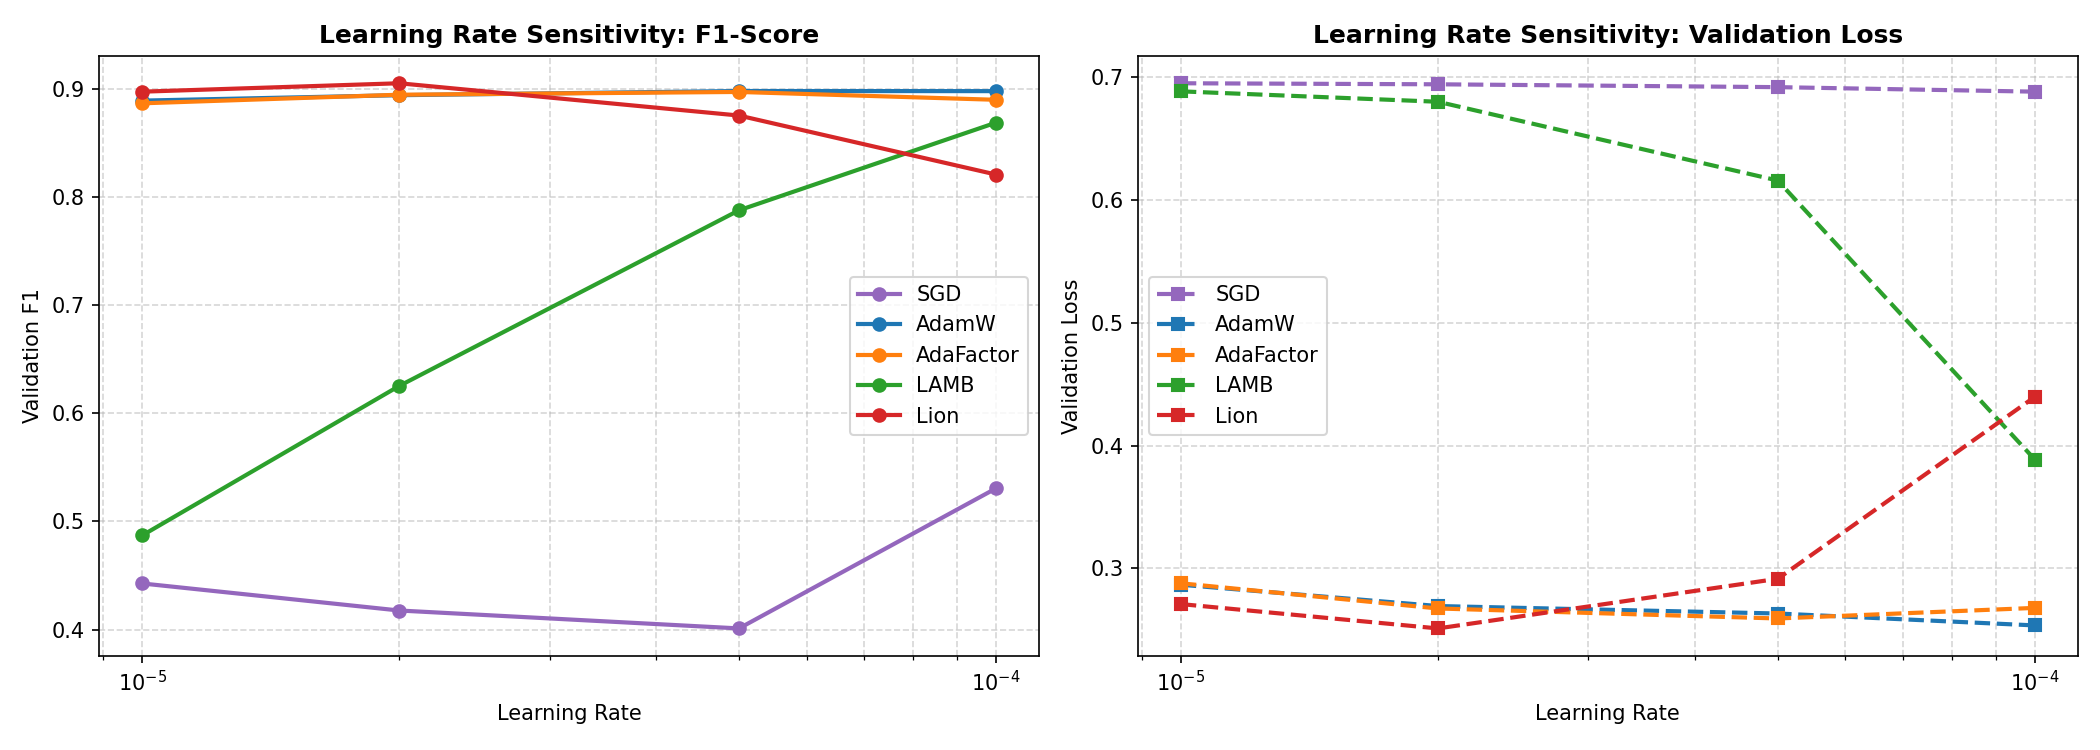
\includegraphics[width=\textwidth, height=0.6\textheight, keepaspectratio]{lr_sensitivity.png}
                \\[4pt]
                \tiny \color{gray} \textit{Figure : Sensibilité F1-Score et Loss selon le LR}
            \end{center}
        \end{column}
    \end{columns}
\end{frame}

% ============================================================
% PAGE 15 : CONTENU — ROBUSTESSE BATCH SIZE
% ============================================================
\begin{frame}{Robustesse au Batch Size}
    \vspace{0.1cm}
    \begin{columns}[c]
        \begin{column}{0.42\textwidth}
            \begin{block}{\faMemory\quad Résultats Clés}
                \scriptsize
                \textbf{AdaFactor} : meilleure performance avec la \textbf{mémoire la plus faible}, à toutes les tailles (8, 16, 32).
                \\[6pt]
                \textbf{LAMB \& SGD} : chute fortement sur petits batchs.
            \end{block}
        \end{column}

        \begin{column}{0.56\textwidth}
            \begin{center}
                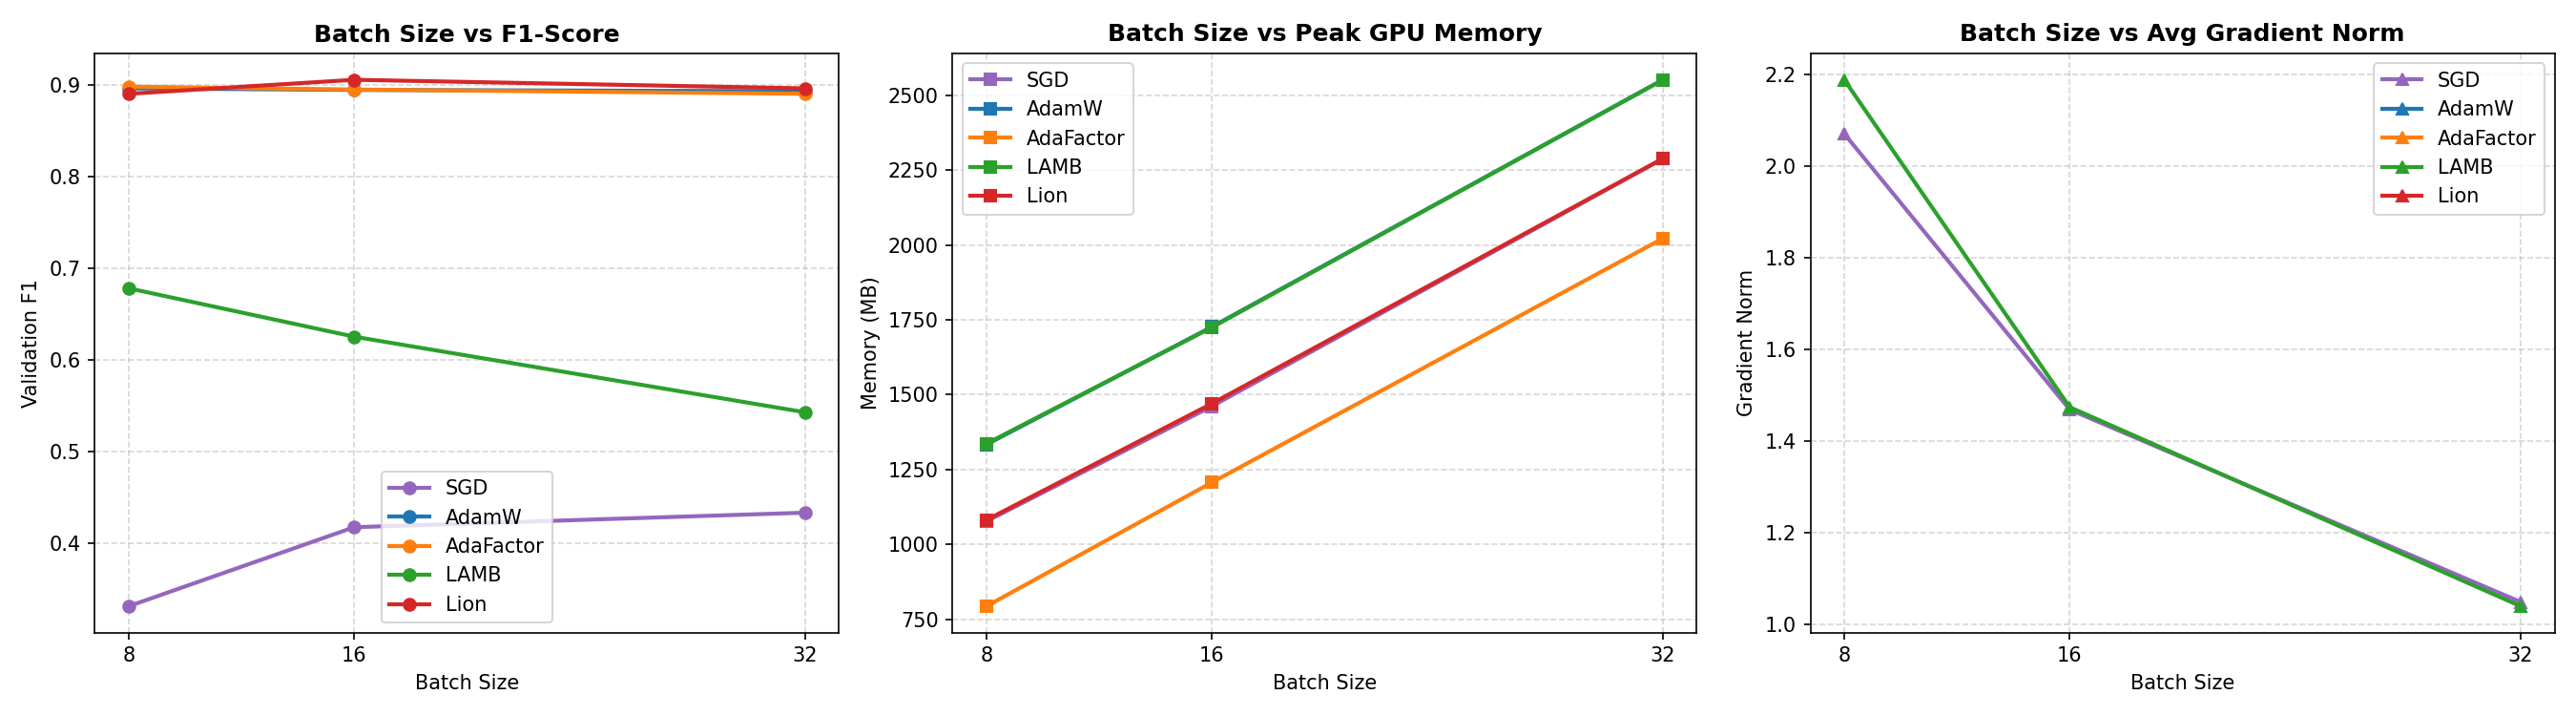
\includegraphics[width=\textwidth, height=0.6\textheight, keepaspectratio]{batch_size_stability.png}
                \\[4pt]
                \tiny \color{gray} \textit{Figure : Robustesse F1 / mémoire selon le batch size}
            \end{center}
        \end{column}
    \end{columns}
\end{frame}

% ============================================================
% PAGE 16 : DISCUSSION + CONCLUSION FUSIONNÉE
% ============================================================
\section{Conclusion \& Recommandations}
\begin{frame}{Conclusion \& Recommandations}
    \vspace{0.1cm}
    \begin{columns}[t]
        \begin{column}{0.48\textwidth}
            \begin{block}{\faFlag\quad Réalisations Clés}
                \scriptsize
                \begin{itemize}
                    \setlength{\itemsep}{4pt}
                    \item[\color{StartupCyan}\faCheck] 5 optimiseurs comparés sous protocole strict
                    \item[\color{StartupCyan}\faCheck] Analyses de sensibilité LR \& batch size
                    \item[\color{StartupCyan}\faCheck] Suivi des gradients par couche
                    \item[\color{StartupCyan}\faCheck] Pipeline 100\% reproductible (seed=42)
                \end{itemize}
            \end{block}
        \end{column}

        \begin{column}{0.48\textwidth}
            \begin{alertblock}{\faTrophy\quad Recommandation Finale}
                \scriptsize
                \textbf{AdaFactor} : meilleur compromis pour GPU limité (F1=89.72\%, -30\% mémoire vs AdamW).
                \\[6pt]
                \textbf{AdamW} : choix sûr et stable par défaut.
                \\[6pt]
                \textbf{Perspective} : valider sur MiniLM.
            \end{alertblock}
        \end{column}
    \end{columns}
    \vspace{0.4cm}
    \begin{center}
        {\footnotesize \color{StartupBlue} \faGithub \quad \texttt{github.com/BOULATARM/projet16-adaptive-gradient-methods-nlp}}
    \end{center}
    \vspace{0.2cm}
\end{frame}
% ============================================================
% PAGE 17 : REMERCIEMENTS
% ============================================================
\begin{frame}[plain]
    \begin{tikzpicture}[remember picture, overlay]
        \fill[white] (current page.south west) rectangle (current page.north east);

        \node[fill=StartupBlue!8, text=StartupBlue, rounded corners=3pt, inner sep=4pt, font=\bfseries\tiny]
            at ([yshift=2.6cm]current page.center)
            {FIN DE LA PRÉSENTATION};

        \node[anchor=center, text width=0.85\textwidth, align=center]
            at ([yshift=1.3cm]current page.center) {
            {\Huge \bfseries \color{StartupBlue} Merci pour\ votre} \\[4pt]
            {\Huge \bfseries \color{StartupCyan} Attention\ !}
        };

        \draw[StartupCyan, line width=2pt] ([xshift=-1.5cm, yshift=0.05cm]current page.center) -- ([xshift=1.5cm, yshift=0.05cm]current page.center);

        \node[anchor=north, text width=0.8\textwidth, align=center]
            at ([yshift=-0.2cm]current page.center) {
            {\small \color{gray!60!black} Place à présent à vos questions et remarques}
        };

        \node[anchor=north, text width=0.9\textwidth, align=center]
            at ([yshift=-1.1cm]current page.center) {
            {\footnotesize \color{StartupBlue} \faGithub \quad \texttt{github.com/BOULATARM/projet16-adaptive-gradient-methods-nlp}}
        };

        \node[anchor=south west, text width=0.45\textwidth, align=left]
            at ([xshift=0.8cm, yshift=0.35cm]current page.south west) {
            {\scriptsize \color{gray} \faUserGraduate \quad Groupe 16 :} \\[2pt]
            {\small \bfseries \color{StartupBlue} Mouad BOULATAR, Mohamed Amine GHAZLI,} \\
            {\small \bfseries \color{StartupBlue} Ayoub HAMROUDI, Jad MOUSLIM}
        };

        \node[anchor=south east, text width=0.35\textwidth, align=right]
            at ([xshift=-0.8cm, yshift=0.35cm]current page.south east) {
            {\scriptsize \color{gray} \faUserTie \quad Supervisé par :} \\[2pt]
            {\small \bfseries \color{StartupBlue} Pr. Faouzia BENABBOU}
        };
    \end{tikzpicture}
\end{frame}

\end{document}